\documentclass[aspectratio=169]{beamer}
\usetheme{Madrid}
\usecolortheme{default}

\usepackage{graphicx}
\usepackage{listings}
\usepackage{xcolor}
\usepackage{amsmath}
\usepackage{tikz}
\usetikzlibrary{positioning,shapes,arrows}
\usepackage{booktabs}
\usepackage{multirow}
\usepackage{hyperref}

% Code listing style
\lstset{
    language=Python,
    basicstyle=\ttfamily\footnotesize,
    keywordstyle=\color{blue},
    commentstyle=\color{green!60!black},
    stringstyle=\color{red},
    showstringspaces=false,
    breaklines=true,
    frame=single,
    numbers=left,
    numberstyle=\tiny\color{gray}
}

\title[System Threat Forecaster]{System Threat Forecaster: Complete Technical Workflow}
\subtitle{Machine Learning \& Deep Learning Approaches}
\author{Technical Documentation}
\date{\today}

\begin{document}

% Title Slide
\begin{frame}
    \titlepage
\end{frame}

% Table of Contents
\begin{frame}[shrink=5]{Agenda}
    \tableofcontents
\end{frame}

\section{Project Overview}

\begin{frame}{Project Overview}
    \begin{block}{Objective}
        Predict potential malware infections in computer systems using machine learning and deep learning approaches
    \end{block}
    
    \vspace{0.5cm}
    
    \begin{columns}[T]
        \begin{column}{0.48\textwidth}
            \textbf{Dataset:}
            \begin{itemize}
                \item 100,000 training samples
                \item 76 features (48 numeric, 28 categorical)
                \item Binary classification (malware vs clean)
                \item Balanced classes: 50.52\% malware, 49.48\% clean
            \end{itemize}
        \end{column}
        
        \begin{column}{0.48\textwidth}
            \textbf{Approaches:}
            \begin{itemize}
                \item Traditional ML: 7 algorithms
                \item Deep Learning: 6 neural architectures
                \item Modular pipeline design
                \item Production-ready implementation
            \end{itemize}
        \end{column}
    \end{columns}
\end{frame}

\begin{frame}{Key Features}
    \small
    \begin{enumerate}
        \item \textbf{Modular Architecture}: Independent components
        \item \textbf{Multiple Models}: Compare 7 ML + 6 DL algorithms
        \item \textbf{Automated Pipeline}: End-to-end workflow
        \item \textbf{Flexible Configuration}: Central CONFIG system
        \item \textbf{Comprehensive Logging}: Track experiments
        \item \textbf{Web App Integration}: Deployment-ready models
    \end{enumerate}
\end{frame}

\section{Machine Learning Workflow}

\begin{frame}[shrink=10]{ML Workflow: Architecture Overview}
    \begin{center}
        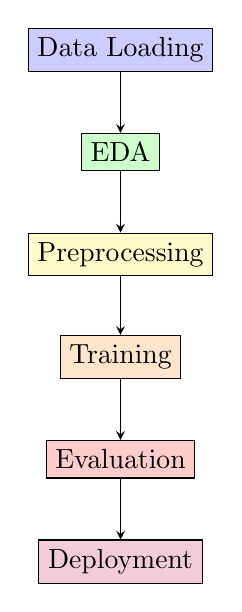
\begin{tikzpicture}[node distance=1.3cm, auto, >=stealth]
            \node[draw, rectangle, fill=blue!20] (load) {Data Loading};
            \node[draw, rectangle, fill=green!20, below of=load] (eda) {EDA};
            \node[draw, rectangle, fill=yellow!20, below of=eda] (preprocess) {Preprocessing};
            \node[draw, rectangle, fill=orange!20, below of=preprocess] (train) {Training};
            \node[draw, rectangle, fill=red!20, below of=train] (eval) {Evaluation};
            \node[draw, rectangle, fill=purple!20, below of=eval] (deploy) {Deployment};
            
            \draw[->] (load) -- (eda);
            \draw[->] (eda) -- (preprocess);
            \draw[->] (preprocess) -- (train);
            \draw[->] (train) -- (eval);
            \draw[->] (eval) -- (deploy);
        \end{tikzpicture}
    \end{center}
\end{frame}

\subsection{Environment Setup}

\begin{frame}[fragile]{ML: Environment Setup}
    \begin{lstlisting}
import numpy as np, pandas as pd
from sklearn.preprocessing import StandardScaler, LabelEncoder
from sklearn.model_selection import train_test_split
from sklearn.metrics import classification_report, accuracy_score
from sklearn.ensemble import RandomForestClassifier
from lightgbm import LGBMClassifier
    \end{lstlisting}
    
    \vspace{0.2cm}
    \small
    \begin{block}{Key Libraries}
        \textbf{Scikit-learn} (ML algorithms), \textbf{LightGBM} (best performer), \textbf{Pandas/NumPy} (data), \textbf{Matplotlib} (visualization)
    \end{block}
\end{frame}

\subsection{Configuration}

\begin{frame}[fragile,shrink=10]{ML: Configuration System}
    \begin{lstlisting}
CONFIG = {
    'data_path': {'train': './kaggle/input/train.csv',
                  'test': './kaggle/input/test.csv'},
    'run_eda': True,
    'models_to_train': {
        'decision_tree': True,
        'random_forest': True,
        'lightgbm': True,  # Best performer
        'ada_boost': True
    },
    'random_state': 42
}
    \end{lstlisting}
\end{frame}

\begin{frame}{ML: Configuration Benefits}
    \begin{block}{Centralized Control}
        Single point to enable/disable pipeline components
    \end{block}
    
    \begin{columns}[T]
        \begin{column}{0.48\textwidth}
            \textbf{Data Pipeline Control:}
            \begin{itemize}
                \item File paths
                \item Missing value handling
                \item Feature engineering
                \item Feature selection
                \item Dimensionality reduction
            \end{itemize}
        \end{column}
        
        \begin{column}{0.48\textwidth}
            \textbf{Model Selection:}
            \begin{itemize}
                \item 7 algorithms available
                \item Easy enable/disable
                \item Hyperparameter tuning
                \item Cross-validation folds
                \item Train-test split ratio
            \end{itemize}
        \end{column}
    \end{columns}
\end{frame}

\subsection{Utility Functions}

\begin{frame}[fragile]{ML: Utility Functions}
    \begin{lstlisting}
def load_data(path):
    return pd.read_csv(path)

def save_model(model, model_name):
    timestamp = datetime.now().strftime("%Y%m%d_%H%M%S")
    filename = f"models/{model_name}_{timestamp}.joblib"
    joblib.dump(model, filename)

def log_result(model_name, metrics, hyperparams=None):
    log_data = {'model_name': model_name,
                'accuracy': metrics['accuracy'],
                'timestamp': datetime.now()}
    df.to_csv('results/model_comparison.csv', mode='a')
    \end{lstlisting}
\end{frame}

\begin{frame}{ML: Utility Benefits}
    \small
    \begin{enumerate}
        \item \textbf{Data Management}: Consistent loading, error handling
        \vspace{0.2cm}
        \item \textbf{Model Persistence}: Timestamped files for versioning
        \vspace{0.2cm}
        \item \textbf{Results Logging}: Performance tracking and model selection
    \end{enumerate}
\end{frame}

\subsection{Exploratory Data Analysis}

\begin{frame}{ML: EDA Overview}
    \begin{block}{Purpose}
        Understand dataset characteristics to guide preprocessing and model selection
    \end{block}
    
    \vspace{0.5cm}
    
    \begin{columns}[T]
        \begin{column}{0.48\textwidth}
            \textbf{Dataset Analysis:}
            \begin{itemize}
                \item Shape: 100,000 × 76
                \item Data types identification
                \item Missing value patterns
                \item Statistical summaries
            \end{itemize}
        \end{column}
        
        \begin{column}{0.48\textwidth}
            \textbf{Feature Analysis:}
            \begin{itemize}
                \item Distribution plots
                \item Correlation heatmap
                \item Target variable balance
                \item Top correlated features
            \end{itemize}
        \end{column}
    \end{columns}
\end{frame}

\begin{frame}{ML: Key EDA Findings}
    \small
    \begin{itemize}
        \item \textbf{Features}: 48 numeric, 28 categorical
        \item \textbf{Target}: Balanced (50.52\% vs 49.48\%)
        \item \textbf{Missing Values}: Several columns affected
        \item \textbf{Top Correlations}: AntivirusConfigID (0.118), TotalPhysicalRAMMB (0.066)
        \item \textbf{Insight}: Moderate correlations → ensemble models needed
    \end{itemize}
\end{frame}

\subsection{Data Preprocessing}

\begin{frame}{ML: Preprocessing Pipeline}
    \small
    \begin{enumerate}
        \item \textbf{Feature Separation}: Split X, y and identify column types
        \vspace{0.2cm}
        \item \textbf{Missing Values}: Mean (numeric), mode (categorical)
        \vspace{0.2cm}
        \item \textbf{Encoding}: LabelEncoder for categorical features
        \vspace{0.2cm}
        \item \textbf{Scaling}: StandardScaler: $z = \frac{x - \mu}{\sigma}$
    \end{enumerate}
\end{frame}

\begin{frame}[fragile]{ML: Preprocessing Code}
    \small
    \begin{lstlisting}
def preprocess_data(data, is_training=True):
    X = data.drop('target', axis=1)
    y = data['target']
    
    numeric_cols = X.select_dtypes(include=['int64']).columns
    categorical_cols = X.select_dtypes(include=['object']).columns
    
    X[numeric_cols] = SimpleImputer(strategy='mean').fit_transform(X[numeric_cols])
    X[categorical_cols] = SimpleImputer(strategy='most_frequent').fit_transform(X[categorical_cols])
    
    X = LabelEncoder().fit_transform(X)
    X_scaled = StandardScaler().fit_transform(X)
    
    return X_scaled, y
    \end{lstlisting}
\end{frame}

\subsection{Feature Engineering \& Selection}

\begin{frame}{ML: Optional Feature Processing}
    \small
    \begin{block}{Feature Engineering (Disabled)}
        Creates interaction features (e.g., AntivirusConfigID × TotalPhysicalRAMMB)
    \end{block}
    \vspace{0.2cm}
    \begin{block}{Feature Selection (Disabled)}
        SelectKBest with ANOVA F-test keeps top 30 features
    \end{block}
    \vspace{0.2cm}
    \begin{block}{Dimensionality Reduction (Disabled)}
        PCA with 95\% variance → $\sim$40 components
    \end{block}
\end{frame}

\subsection{Model Training}

\begin{frame}[shrink=5]{ML: Seven Algorithms Implemented}
    \begin{table}
        \centering
        \begin{tabular}{lcc}
            \toprule
            \textbf{Model} & \textbf{Accuracy} & \textbf{Type} \\
            \midrule
            LightGBM & \textcolor{green}{\textbf{63.0\%}} & Gradient Boosting \\
            Random Forest & 62.4\% & Ensemble (Bagging) \\
            AdaBoost & 62.0\% & Ensemble (Boosting) \\
            Decision Tree & $\sim$60\% & Single Tree \\
            Logistic Regression & $\sim$60\% & Linear Model \\
            Naive Bayes & Lower & Probabilistic \\
            SGD & Lower & Online Learning \\
            \bottomrule
        \end{tabular}
    \end{table}
    
    \vspace{0.2cm}
    
    \begin{alertblock}{Best Model}
        \textbf{LightGBM} achieves 63.0\% accuracy due to:
        \begin{itemize}
            \item Leaf-wise tree growth (vs level-wise)
            \item Handles large datasets efficiently
            \item Built-in categorical feature support
        \end{itemize}
    \end{alertblock}
\end{frame}

\begin{frame}[fragile,shrink=10]{ML: Training Process}
    \footnotesize
    \begin{lstlisting}
def train_model(model_name, X_train, y_train, X_val, y_val):
    params = get_default_model_params(model_name)
    
    model = get_model(model_name, params)
    model.fit(X_train, y_train)
    
    val_pred = model.predict(X_val)
    metrics = {
        'val_accuracy': accuracy_score(y_val, val_pred),
        'precision': precision_score(y_val, val_pred),
        'f1_score': f1_score(y_val, val_pred)
    }
    
    save_model(model, model_name)
    return model, metrics
    \end{lstlisting}
\end{frame}

\begin{frame}[shrink=5]{ML: Evaluation Metrics}
    \begin{columns}[T]
        \begin{column}{0.48\textwidth}
            \textbf{Accuracy}:
            $$\frac{\text{Correct Predictions}}{\text{Total Predictions}}$$
            
            \vspace{0.3cm}
            
            \textbf{Precision}:
            $$\frac{\text{True Positives}}{\text{True Positives} + \text{False Positives}}$$
        \end{column}
        
        \begin{column}{0.48\textwidth}
            \textbf{Recall}:
            $$\frac{\text{True Positives}}{\text{True Positives} + \text{False Negatives}}$$
            
            \vspace{0.3cm}
            
            \textbf{F1-Score}:
            $$2 \cdot \frac{\text{Precision} \cdot \text{Recall}}{\text{Precision} + \text{Recall}}$$
        \end{column}
    \end{columns}
    
    \vspace{0.3cm}
    
    \begin{block}{Confusion Matrix}
        Visualizes True Positives, False Positives, True Negatives, False Negatives
    \end{block}
\end{frame}

\subsection{ML Pipeline Execution}

\begin{frame}{ML: Complete Pipeline Flow}
    \small
    \begin{enumerate}
        \item Load \texttt{train.csv} and \texttt{test.csv}
        \item Run EDA and preprocess (handle missing, encode, scale)
        \item Split train (80\%) / validation (20\%)
        \item Optional: Feature engineering, selection, PCA
        \item Train all selected models (7 algorithms)
        \item Compare performance and select best
        \item Generate predictions and save models
        \item Export metrics to \texttt{results/model\_performance.json}
    \end{enumerate}
\end{frame}

\begin{frame}{ML: Output Files}
    \begin{table}
        \centering
        \begin{tabular}{ll}
            \toprule
            \textbf{File} & \textbf{Purpose} \\
            \midrule
            \texttt{saved\_models/ml\_models.pkl} & All trained models \\
            \texttt{saved\_models/preprocessors.pkl} & Scalers, encoders \\
            \texttt{results/model\_comparison.csv} & Performance log \\
            \texttt{results/model\_performance.json} & Structured metrics \\
            \texttt{submission.csv} & Kaggle submission \\
            \texttt{models/lightgbm\_*.joblib} & Versioned models \\
            \bottomrule
        \end{tabular}
    \end{table}
\end{frame}

\section{Deep Learning Workflow}

\begin{frame}[shrink=10]{DL Workflow: Architecture Overview}
    \begin{center}
        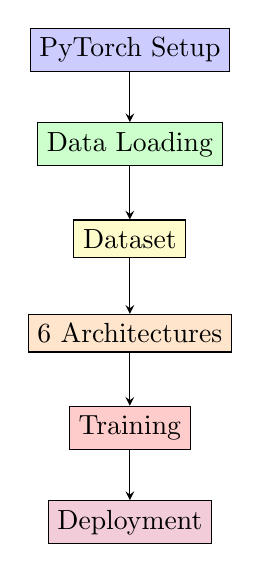
\begin{tikzpicture}[node distance=1.2cm, auto, >=stealth]
            \node[draw, rectangle, fill=blue!20] (setup) {PyTorch Setup};
            \node[draw, rectangle, fill=green!20, below of=setup] (data) {Data Loading};
            \node[draw, rectangle, fill=yellow!20, below of=data] (dataset) {Dataset};
            \node[draw, rectangle, fill=orange!20, below of=dataset] (arch) {6 Architectures};
            \node[draw, rectangle, fill=red!20, below of=arch] (train) {Training};
            \node[draw, rectangle, fill=purple!20, below of=train] (deploy) {Deployment};
            
            \draw[->] (setup) -- (data);
            \draw[->] (data) -- (dataset);
            \draw[->] (dataset) -- (arch);
            \draw[->] (arch) -- (train);
            \draw[->] (train) -- (deploy);
        \end{tikzpicture}
    \end{center}
\end{frame}

\subsection{PyTorch Setup}

\begin{frame}[fragile]{DL: Environment Setup}
    \small
    \begin{lstlisting}
import torch, torch.nn as nn
from torch.utils.data import Dataset, DataLoader

torch.manual_seed(42)  # Reproducibility

# Device detection (GPU acceleration)
if torch.cuda.is_available():
    device = torch.device('cuda')  # NVIDIA
elif torch.backends.mps.is_available():
    device = torch.device('mps')   # Apple Silicon
else:
    device = torch.device('cpu')   # CPU
    \end{lstlisting}
    \vspace{0.2cm}
    \begin{alertblock}{GPU Acceleration}
        CUDA (10-100×), MPS (5-15×), CPU (1×)
    \end{alertblock}
\end{frame}

\subsection{DL Configuration}

\begin{frame}[fragile,shrink=10]{DL: Configuration}
    \begin{lstlisting}
CONFIG = {
    'batch_size': 512,
    'epochs': 100,
    'learning_rate': 0.001,
    'hidden_dims': [256, 128, 64, 32],
    'dropout_rate': 0.3,
    'use_batch_norm': True,
    'optimizer': 'adamw',
    'use_mixed_precision': torch.cuda.is_available()
}
    \end{lstlisting}
\end{frame}

\begin{frame}{DL: Configuration Comparison}
    \begin{table}
        \centering
        \small
        \begin{tabular}{lll}
            \toprule
            \textbf{Setting} & \textbf{ML} & \textbf{DL} \\
            \midrule
            Training & One-shot \texttt{.fit()} & Iterative epochs \\
            Batch Size & N/A & 512 \\
            Learning Rate & N/A & 0.001 \\
            Regularization & N/A & Dropout (0.3) \\
            Data Format & DataFrame & Tensors \\
            Feature Eng. & Manual & Automatic \\
            Computation & CPU & GPU-accelerated \\
            Training Time & Minutes & Hours \\
            \bottomrule
        \end{tabular}
    \end{table}
\end{frame}

\subsection{PyTorch Dataset}

\begin{frame}[fragile,shrink=10]{DL: Custom Dataset Class}
    \small
    \begin{lstlisting}
class TabularDataset(Dataset):
    def __init__(self, X, y=None):
        self.X = torch.FloatTensor(X)
        self.y = torch.LongTensor(y) if y else None
    
    def __len__(self): return len(self.X)
    def __getitem__(self, idx):
        return (self.X[idx], self.y[idx]) if self.y else self.X[idx]

train_loader = DataLoader(train_dataset, batch_size=512,
                          shuffle=True, num_workers=4)
    \end{lstlisting}
\end{frame}

\begin{frame}{DL: DataLoader Benefits}
    \small
    \begin{enumerate}
        \item \textbf{Batching}: Groups 512 samples, memory efficient
        \vspace{0.2cm}
        \item \textbf{Shuffling}: Prevents order patterns, improves generalization
        \vspace{0.2cm}
        \item \textbf{Parallel Loading}: 4 workers eliminate bottleneck
        \vspace{0.2cm}
        \item \textbf{Class Imbalance}: Weighted loss [1.98, 2.02]
    \end{enumerate}
\end{frame}

\subsection{Neural Network Architectures}

\begin{frame}{DL: Six Architectures}
    \begin{table}
        \centering
        \small
        \begin{tabular}{lccc}
            \toprule
            \textbf{Model} & \textbf{Accuracy} & \textbf{Time} & \textbf{Params} \\
            \midrule
            Simple MLP & 60-62\% & 5 min & 50K \\
            Deep MLP & 62-64\% & 10 min & 100K \\
            Residual Net & 63-65\% & 15 min & 200K \\
            Attention Net & 64-66\% & 20 min & 300K \\
            Wide \& Deep & 63-65\% & 12 min & 150K \\
            FT-Transformer & \textcolor{green}{\textbf{65-68\%}} & 30 min & 500K \\
            \bottomrule
        \end{tabular}
    \end{table}
    
    \vspace{0.3cm}
    
    \begin{alertblock}{Best Architecture}
        \textbf{FT-Transformer}: 4-5\% improvement over traditional ML
    \end{alertblock}
\end{frame}

\begin{frame}{Architecture 1: Simple MLP}
    \begin{columns}[T]
        \begin{column}{0.48\textwidth}
            \textbf{Structure}:
            \begin{itemize}
                \item Input (76 features)
                \item Linear(76 → 256) + ReLU + Dropout
                \item Linear(256 → 128) + ReLU + Dropout
                \item Linear(128 → 64) + ReLU + Dropout
                \item Output(64 → 2)
            \end{itemize}
        \end{column}
        
        \begin{column}{0.48\textwidth}
            \textbf{Components}:
            \begin{itemize}
                \item \textbf{Linear}: $y = Wx + b$
                \item \textbf{ReLU}: $\max(0, x)$
                \item \textbf{Dropout}: Zeros 30\% neurons
            \end{itemize}
            
            \vspace{0.5cm}
            
            \textbf{Use Case}:
            \begin{itemize}
                \item Baseline model
                \item Fast training
                \item 60-62\% accuracy
            \end{itemize}
        \end{column}
    \end{columns}
\end{frame}

\begin{frame}[fragile,shrink=5]{Architecture 2: Deep MLP with Batch Norm}
    \small
    \begin{lstlisting}
class DeepMLP(nn.Module):
    def __init__(self, input_dim, hidden_dims=[256, 128, 64]):
        super().__init__()
        layers = []
        for hidden_dim in hidden_dims:
            layers.append(nn.Linear(prev_dim, hidden_dim))
            layers.append(nn.BatchNorm1d(hidden_dim))
            layers.append(nn.ReLU())
            layers.append(nn.Dropout(0.3))
        self.network = nn.Sequential(*layers)
    \end{lstlisting}
    \vspace{0.1cm}
    \begin{block}{Batch Normalization}
        $$x_{norm} = \frac{x - \mu_{batch}}{\sqrt{\sigma^2_{batch} + \epsilon}}, \quad output = \gamma \cdot x_{norm} + \beta$$
        Faster training, stability (62-64\% accuracy)
    \end{block}
\end{frame}

\begin{frame}[shrink=5]{Architecture 3: Residual Network}
    \small
    \begin{columns}[T]
        \begin{column}{0.48\textwidth}
            \textbf{Skip Connections}:
            \begin{center}
                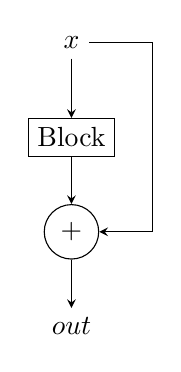
\begin{tikzpicture}[node distance=1.2cm, auto, >=stealth]
                    \node (input) {$x$};
                    \node[draw, rectangle, below of=input] (block1) {Block};
                    \node[draw, circle, below of=block1] (add) {+};
                    \node[below of=add] (output) {$out$};
                    
                    \draw[->] (input) -- (block1);
                    \draw[->] (block1) -- (add);
                    \draw[->] (add) -- (output);
                    \draw[->] (input.east) -- ++(0.8,0) |- (add.east);
                \end{tikzpicture}
            \end{center}
            
            $$out = Block(x) + x$$
        \end{column}
        
        \begin{column}{0.48\textwidth}
            \textbf{Benefits}:
            \begin{itemize}
                \item Solves vanishing gradients
                \item Deeper networks (100+ layers)
                \item 63-65\% accuracy
            \end{itemize}
        \end{column}
    \end{columns}
\end{frame}

\begin{frame}[shrink=5]{Architecture 4: Attention Network}
    \small
    \textbf{Self-Attention}: $\text{Attention}(Q, K, V) = \text{softmax}\left(\frac{QK^T}{\sqrt{d_k}}\right) \cdot V$
    
    \vspace{0.3cm}
    
    \begin{columns}[T]
        \begin{column}{0.48\textwidth}
            \textbf{Mechanism}:
            \begin{itemize}
                \item Each feature attends to others
                \item Learns interactions automatically
            \end{itemize}
        \end{column}
        
        \begin{column}{0.48\textwidth}
            \textbf{Benefits}:
            \begin{itemize}
                \item Complex relationships
                \item Interpretable weights
                \item 64-66\% accuracy
            \end{itemize}
        \end{column}
    \end{columns}
    
    \vspace{0.3cm}
    
    \begin{alertblock}{Innovation}
        Transforms NLP architecture for tabular data
    \end{alertblock}
\end{frame}

\begin{frame}{Architecture 5: Wide \& Deep}
    \begin{columns}[T]
        \begin{column}{0.58\textwidth}
            \textbf{Simplified Architecture:}
            
            \vspace{0.3cm}
            
            Input (76 features) splits into:
            \begin{itemize}
                \item Wide path: Direct Linear(76 $\rightarrow$ 2)
                \item Deep path: MLP 256 $\rightarrow$ 128 $\rightarrow$ 64 $\rightarrow$ 2
            \end{itemize}
            
            \vspace{0.3cm}
            
            Both outputs are added together for final prediction.
        \end{column}
        
        \begin{column}{0.38\textwidth}
            \textbf{Components}:
            \begin{itemize}
                \item \textbf{Wide}: Memorization (frequent patterns)
                \item \textbf{Deep}: Generalization (novel combinations)
            \end{itemize}
            
            \vspace{0.5cm}
            
            \textbf{Use Case}:
            \begin{itemize}
                \item Google Play recommendations
                \item 63-65\% accuracy
            \end{itemize}
        \end{column}
    \end{columns}
\end{frame}

\begin{frame}{Architecture 6: FT-Transformer (Best)}
    \small
    \textbf{Feature Tokenizer Transformer} - SOTA for tabular data
    
    \vspace{0.2cm}
    
    \begin{enumerate}
        \item \textbf{Tokenization}: Each feature → 192-dim vector
        \item \textbf{CLS Token}: Prepend classification token (like BERT)
        \item \textbf{Positional Embeddings}: Learnable position encoding
        \item \textbf{Transformer}: 8-head self-attention, 3 blocks
        \item \textbf{Classification}: CLS token → Linear(192 → 2)
    \end{enumerate}
    
    \vspace{0.2cm}
    
    \begin{alertblock}{Performance}
        \textbf{65-68\% accuracy} - 4-5\% improvement over ML
    \end{alertblock}
\end{frame}

\subsection{Training Process}

\begin{frame}{DL: Training Loop}
    \small
    \begin{enumerate}
        \item \textbf{Forward}: $\hat{y} = f_\theta(x)$ (network prediction)
        \vspace{0.1cm}
        \item \textbf{Loss}: $L = -\log(P(\text{correct class}))$ (CrossEntropy)
        \vspace{0.1cm}
        \item \textbf{Backward}: $\frac{\partial L}{\partial \theta}$ (compute gradients)
        \vspace{0.1cm}
        \item \textbf{Update}: $\theta_{t+1} = \theta_t - \alpha \cdot \nabla_\theta L$ (AdamW)
    \end{enumerate}
    
    \vspace{0.2cm}
    \begin{block}{Iterative Learning}
        Repeat for 100 epochs
    \end{block}
\end{frame}

\begin{frame}[fragile]{DL: Training Code}
    \small
    \begin{lstlisting}
def train_epoch(model, train_loader, criterion, optimizer):
    model.train()
    
    for data, target in train_loader:
        output = model(data)
        loss = criterion(output, target)
        
        optimizer.zero_grad()
        loss.backward()
        optimizer.step()
    
    return avg_loss, accuracy

for epoch in range(100):
    train_loss = train_epoch(...)
    val_loss = validate(...)
    if early_stopping(val_loss): break
    \end{lstlisting}
\end{frame}

\begin{frame}{DL: Advanced Training Techniques}
    \small
    \begin{enumerate}
        \item \textbf{Early Stopping}: Stop if no improvement for 15 epochs
        \vspace{0.2cm}
        \item \textbf{LR Scheduling}: Reduce when stuck (0.001 → 0.0005)
        \vspace{0.2cm}
        \item \textbf{Mixed Precision}: FP16 for 2-3× speedup (NVIDIA)
        \vspace{0.2cm}
        \item \textbf{Checkpointing}: Save best model by validation accuracy
    \end{enumerate}
\end{frame}

\begin{frame}{DL: Complete Pipeline Flow}
    \small
    \begin{enumerate}
        \item Load and preprocess → NumPy arrays
        \item Create DataLoaders (batch size=512)
        \item Split train (80\%) / validation (20\%)
        \item Train 6 architectures (MLP, ResNet, Attention, FT-Transformer)
        \item Evaluate and select best model (FT-Transformer $\sim$67\%)
        \item Generate predictions and save models
        \item Export to \texttt{submission\_dl.csv}
    \end{enumerate}
\end{frame}

\section{Comparison \& Results}

\begin{frame}{ML vs DL: Comprehensive Comparison}
    \begin{table}
        \centering
        \footnotesize
        \begin{tabular}{lll}
            \toprule
            \textbf{Aspect} & \textbf{Machine Learning} & \textbf{Deep Learning} \\
            \midrule
            Best Model & LightGBM (63.0\%) & FT-Transformer (65-68\%) \\
            Training & One-shot \texttt{.fit()} & Iterative epochs \\
            Data Format & DataFrame & Tensors \\
            Feature Eng. & Manual & Automatic \\
            Architecture & Fixed (trees) & Flexible (networks) \\
            Computation & CPU-optimized & GPU-accelerated \\
            Training Time & 5-15 minutes & 30-60 minutes \\
            Interpretability & High & Low (black box) \\
            Hyperparams & Few ($\sim$10) & Many ($\sim$50) \\
            Memory & Low & High (GPU) \\
            \bottomrule
        \end{tabular}
    \end{table}
\end{frame}

\begin{frame}{Performance Summary}
    \begin{table}
        \centering
        \begin{tabular}{lcc}
            \toprule
            \textbf{Category} & \textbf{Model} & \textbf{Accuracy} \\
            \midrule
            \multirow{3}{*}{Traditional ML} & LightGBM & \textcolor{green}{\textbf{63.0\%}} \\
             & Random Forest & 62.4\% \\
             & AdaBoost & 62.0\% \\
            \midrule
            \multirow{3}{*}{Deep Learning} & FT-Transformer & \textcolor{blue}{\textbf{65-68\%}} \\
             & Attention Net & 64-66\% \\
             & Residual Net & 63-65\% \\
            \bottomrule
        \end{tabular}
    \end{table}
    
    \vspace{0.5cm}
    
    \begin{alertblock}{Key Finding}
        Deep Learning achieves \textbf{4-5\% improvement} over traditional ML
    \end{alertblock}
\end{frame}

\begin{frame}{When to Use ML vs DL}
    \begin{columns}[T]
        \begin{column}{0.48\textwidth}
            \textbf{Use Traditional ML When}:
            \begin{itemize}
                \item Small dataset (<10K samples)
                \item Need interpretability
                \item Limited compute resources
                \item Quick prototyping
                \item Tabular data with clear features
                \item Need fast inference
            \end{itemize}
        \end{column}
        
        \begin{column}{0.48\textwidth}
            \textbf{Use Deep Learning When}:
            \begin{itemize}
                \item Large dataset (>50K samples)
                \item Complex patterns
                \item GPU available
                \item Maximum performance needed
                \item Many feature interactions
                \item Time for experimentation
            \end{itemize}
        \end{column}
    \end{columns}
    
    \vspace{0.5cm}
    
    \begin{block}{Our Project}
        With 100K samples and GPU access, DL provides the best performance
    \end{block}
\end{frame}

\section{Web Application Integration}

\begin{frame}{Deployment Pipeline}
    \small
    \begin{enumerate}
        \item \textbf{Model Saving}: ML (7 models), DL (6 architectures), preprocessors
        \vspace{0.2cm}
        \item \textbf{Metadata}: Best model, accuracy, hyperparameters
        \vspace{0.2cm}
        \item \textbf{Web App}: Load preprocessors and best model (FT-Transformer)
        \vspace{0.2cm}
        \item \textbf{Inference}: User input → Preprocess → Model → Prediction
    \end{enumerate}
\end{frame}

\begin{frame}[fragile]{Web App Integration Code}
    \small
    \begin{lstlisting}
import joblib, torch

preprocessors = joblib.load('saved_models/preprocessors.pkl')
checkpoint = torch.load('saved_models/dl_models.pth')
model = checkpoint['best_model']
model.eval()

def predict(input_features):
    X = preprocessors['scaler'].transform([input_features])
    
    with torch.no_grad():
        output = model(torch.FloatTensor(X))
        pred = output.argmax(dim=1).item()
    
    return "Malware" if pred == 1 else "Clean"
    \end{lstlisting}
\end{frame}

\section{Conclusion}

\begin{frame}{Key Achievements}
    \small
    \begin{enumerate}
        \item \textbf{Implementation}: 7 ML + 6 DL algorithms, production-ready
        \vspace{0.2cm}
        \item \textbf{Performance}: ML (63.0\%), DL (65-68\%), 4-5\% improvement
        \vspace{0.2cm}
        \item \textbf{Technical}: GPU acceleration, mixed precision, Transformers
        \vspace{0.2cm}
        \item \textbf{Deployment}: Model versioning, web app, comprehensive logging
    \end{enumerate}
\end{frame}

\begin{frame}{Technical Highlights}
    \begin{block}{Machine Learning}
        \begin{itemize}
            \item Modular configuration system
            \item Multiple algorithm comparison
            \item Comprehensive preprocessing pipeline
            \item Feature engineering capabilities
        \end{itemize}
    \end{block}
    
    \begin{block}{Deep Learning}
        \begin{itemize}
            \item 6 state-of-the-art architectures
            \item Transformer-based approach for tabular data
            \item Advanced training techniques (early stopping, LR scheduling)
            \item GPU acceleration support
        \end{itemize}
    \end{block}
\end{frame}

\begin{frame}{Future Improvements}
    \small
    \begin{enumerate}
        \item \textbf{Ensemble}: Combine ML + DL predictions, stacking
        \vspace{0.2cm}
        \item \textbf{Optimization}: Optuna, Ray Tune, NAS
        \vspace{0.2cm}
        \item \textbf{Features}: Cross-validation, advanced imputation
        \vspace{0.2cm}
        \item \textbf{Deployment}: ONNX export, quantization, A/B testing
    \end{enumerate}
\end{frame}

\begin{frame}{Thank You}
    \begin{center}
        \Large{\textbf{Questions?}}
        
        \vspace{1cm}
        
        \normalsize
        \textbf{Repository Structure:}
        \begin{itemize}
            \item \texttt{system-threat-forecaster-ml.py} - ML Pipeline
            \item \texttt{system-threat-forecaster-dl.py} - DL Pipeline
            \item \texttt{saved\_models/} - Trained models
            \item \texttt{results/} - Performance metrics
            \item \texttt{models/} - Model checkpoints
        \end{itemize}
        
        \vspace{0.5cm}
        
        \textbf{Best Performance:}
        FT-Transformer at 65-68\% accuracy
    \end{center}
\end{frame}

\appendix

\section{Appendix}

\begin{frame}{Appendix: Hyperparameters - LightGBM}
    \begin{table}
        \centering
        \begin{tabular}{ll}
            \toprule
            \textbf{Parameter} & \textbf{Value} \\
            \midrule
            n\_estimators & 200 \\
            learning\_rate & 0.1 \\
            max\_depth & 5 \\
            subsample & 0.6 \\
            colsample\_bytree & 0.8 \\
            min\_child\_samples & 20 \\
            reg\_alpha & 0.1 \\
            reg\_lambda & 0.1 \\
            \bottomrule
        \end{tabular}
    \end{table}
\end{frame}

\begin{frame}{Appendix: Hyperparameters - FT-Transformer}
    \begin{table}
        \centering
        \begin{tabular}{ll}
            \toprule
            \textbf{Parameter} & \textbf{Value} \\
            \midrule
            d\_token & 192 \\
            n\_blocks & 3 \\
            attention\_heads & 8 \\
            attention\_dropout & 0.2 \\
            ffn\_dropout & 0.1 \\
            residual\_dropout & 0.0 \\
            learning\_rate & 0.001 \\
            weight\_decay & 1e-5 \\
            batch\_size & 512 \\
            epochs & 100 \\
            \bottomrule
        \end{tabular}
    \end{table}
\end{frame}

\begin{frame}{Appendix: Dataset Features}
    \begin{columns}[T]
        \begin{column}{0.48\textwidth}
            \textbf{Numeric Features (48)}:
            \begin{itemize}
                \item TotalPhysicalRAMMB
                \item AvailablePhysicalRAMMB
                \item ProcessorCount
                \item SystemVolumeTotalCapacity
                \item SystemDriveFreeSpace
                \item ...
            \end{itemize}
        \end{column}
        
        \begin{column}{0.48\textwidth}
            \textbf{Categorical Features (28)}:
            \begin{itemize}
                \item AntivirusConfigID
                \item FirewallConfigID
                \item OSVersion
                \item CountryIdentifier
                \item LocaleEnglishName
                \item ...
            \end{itemize}
        \end{column}
    \end{columns}
    
    \vspace{0.5cm}
    
    \textbf{Target Variable}: Binary (0=Clean, 1=Malware)
\end{frame}

\end{document}
